\section{Background and Related Work}
\label{sec:background}
\subsection{Bitcoin}

\textbf{Transaction}

\subsection{Scams in Bitcoin}

Scam in bitcoin refers to fraudulent business or scheme that takes money or other goods from an unsuspected person. There has been different taxonomies towards bitcoin scams. Vasek et al \cite{vasek2015there} categorized scams into Ponzi schemes, mining scams, scam wallets and fradulent exchanges. However, new schemes continuously appear, and the distribution in scams varies a lot. DW-VA Taxonomy\cite{dwva} is a collaborative community activity which aims at providing a scheme for data exchange and analysis for tools and datasets involving artifacts from Dark Web and Virtual Assets. They defines common forms of abuses encountered in Darknet and Cryptoasset investigation as: Scam, Sextortion, Phishing, Service Hack, Ransomware, Ponzi Scheme.

In this paper, in order to make it more comprehensive, we took the above taxonomies into consideration and provided elaboration about some schemes.

%will category scams into several types: ransomeware, darknet market, bitcoin tumbler, blackmail scam, sextortion and other. The category is given by bitcoinabuse.com\cite{bitcoinabuse}. Now we will elaborate each category.
\textbf{Sextortion}
Sextortion is the most popular form in bitcoin scams. The word sextortion is a combination of sex and extortion. In the bitcoin ecosystem, the abuser generally tries to extort money from victim by threatening sending the compromising photos or videos(which under most circumstances, they don't have any) to the victim's contracts, unless a ransom is paid. Masarah et al \cite{paquet2019spams} tracked and investigated monetary flows between involved actors and gain insights into the financial structure of sextortion campaigns.



\textbf{Ransomware}
Generally, ransomware is a type of malware which is typically carried out using a Trojan disguised as a legitimate file and trick user into downloading or opening when it arrives as an email attachment, then it will threatens to publish the victim's data or block access to local files unless certain amount of ransom is paid. Wannacry\cite{wannacry} is a famous example. Wannacry uses EternalBlue, which is an exploit discovered by the NSA to gain access, and then encrypt the data and ask for ransom payment in bitcoin. It infected more than 230,000 computers.

\textbf{Ponzi Scheme}
Ponzi scheme is a famous form of fraud. They don't have real products or investment, but simply lures investors with high profits, and then pays earlier investors with funds from recent investors \cite{vasek2018analyzing}. This scheme has appeared in bitcoin.
\textbf{darknet market Scam}
The term darknet is getting more familiar with people these days. Opposite to clearet, which is the publicly accessible internet, darknet is an overlay network which can only be accessed by those who have specific software, configurations, or authorizations, and there might need a unique customised communication protocol. On the one hand, darknet can provide security, anonymity to avoid censorship. However, on the other hand, darknet can be used by criminals to conduct illegal activities, such as selling drugs, firearms, stolen information etc. So here comes one of the most common scam in darknet, exit scam. After buyers pay in bitcoin, in a normal trade scheme, the seller will then ship the parcels of goods listed above to the buyers. While in an exit scam, the vendor might not mail the goods at all, but simply pocket customer's payments. A number of darkweb scam vendors and market is listed in a thread in dark web magazine. \cite{darkweb-scam-list}.



\textbf{bitcoin tumbler}
\label{bitcoin-tumbler}
A bitcoin tumbler, also known as bitcoin mixer, is a service that mixes bitcoin to obscure their origin. Tumblers take a percentage transaction fee of the total coins mixed to earn a profit. Although bitcoin is anonymous theoretically, 
if the bitcoin wallet user relates the wallet address to a specific account containing identifiable information, for example is the exchange implements Know Your Customer(KYC), then the address may be linked to a real-world identity, the user is no longer anonymous. Besides, the blockchain ledger is completely open, so a map can be created as time goes on that allows analytical tools to find out where bitcoins are going. While anonymity is an important part among bitcoin users, for example, big companies want to make their transaction private so that their 
rival will not have a clue about their commercial strategy. Some bitcoin holder who cares a lot about privacy simply don't want others to know about where they spend their coins. there are also some situations such as donation which requires anonymity.

There are a number of mixing strategies, in centralized bitcoin mixer as shown in \ref{fig:mixer}, all users trust a mixer, the user who want to mix bitcoin will initiate a transaction to send the mixer a certain amount of bitcoins, then, the mixer will match different addresses with different amounts, and sends random amounts of bitcoins to each address until the total amount requested is achieved.

% A graph explaining all this
\begin{figure}[tbp]
\centerline{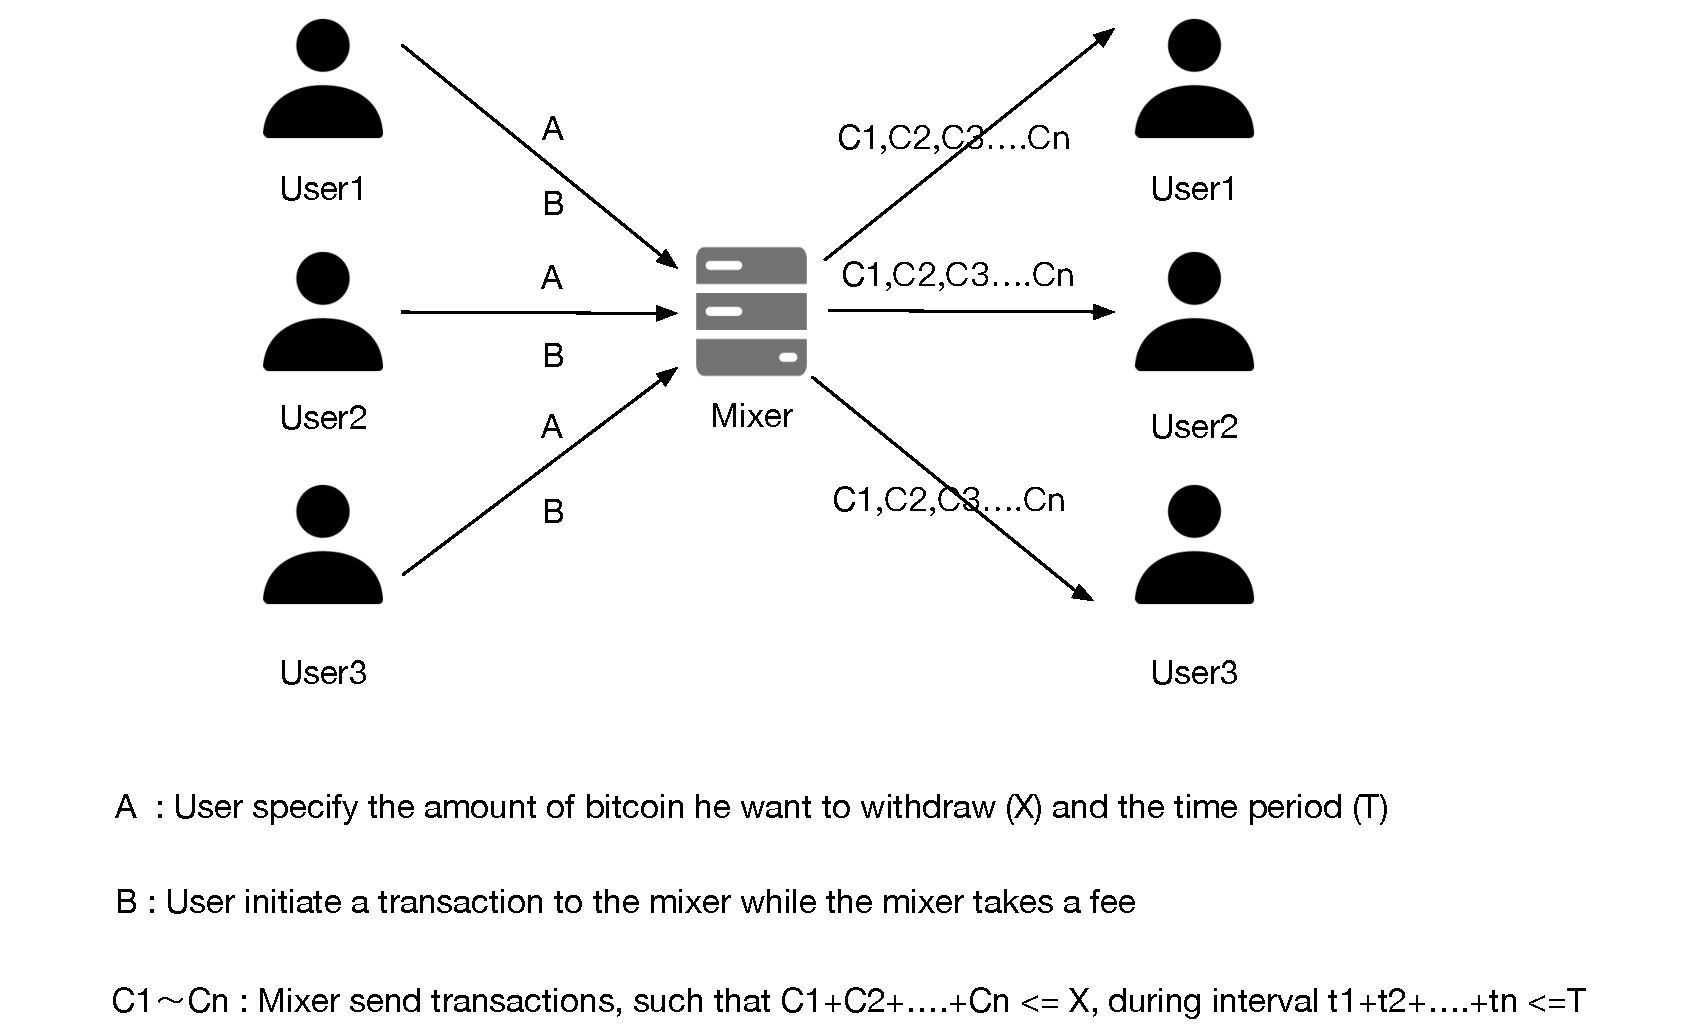
\includegraphics[width=\columnwidth]{images/mixer.pdf}}
\caption{The description of mixer}
\label{fig:mixer}
\end{figure}

There is a bitcointalk thread with some bitcoin tumbler scam urls.\cite{tumbler-scam}:

\textbf{Blackmail Scam}

Scammers will send e-mails to people, claiming to have some of  the handles of the people. If certain amount of ransom is not paid, the scammer will release the handles to the victim's contact. Here is an example:

\textit{I run a site in deepweb,I produce all kinds of services in the main it is demolition to bussiness and injury.In general all but murder.Often this happens because of rejected love or competition at bussiness.This month he contacted me and gave me the mission of pour out sourness in your visage.Default order fast,painfully,for life.Without too much fuss.I get money only after finishing task.Thus now I offer you send money to me to be inactive,I propose this to almost all victims.If I do not get money from you,then my performer will fulfill the order.If you transfer me money,besides to my inaction,I will give you info that I have about the customer.After finishing task I always waist the performer,so I have a selection,to get \$1300 from you for info about the customer and my inaction,or to receive \$5000 from the customer,but with a big probability of losing the performer my BTC address 1ApsrLsKGwfQeEevLFaVjunNUrNnXSNKGy Two days to decide and pay, and bear in mind that time is ticking}

\textbf{Scam coins}
Scam coins lies in altcoins(alternative coins), they will boast about their large community, high profit, and victims may fear about losing a great opportunity to earn some money, so they will buy in, but eventually they will only lose money.

\textbf{Fake exchange and wallet}
Fake exchanges may offer competitive market price to lure user into using them, however, once the user deposit bitcoin into the exchange, they will charge a unreasonale amount of transaction fee, or they might even simply ignore the user and took their money away.

\subsection{Bitcoin Scam Characterizing}
Xia et al.\cite{xia2020characterizing}identified and characterized the cryptocurrency exchange scams, They found 94 scam domain families and 30 fake app families. Paquet-Clouston et al.\cite{paquet2019spams}characterized sextortion in the bitcoin ecosystem and uncovered scammers' operations. Vasek et al.\cite{vasek2018analyzing} characterized Ponzi scheme in bitcoin. However, by far there is no work on characterizing all kinds of scams together.
\subsection{Money flow tracing and graph analysis}
\textbf{UTXO} 
There are two popular ways to keep record in blockchain network. Account/Balance model is used in Ethereum, while bitcoin employs UTXO, which means unspent transaction output. All of the unspent transactions are kept in each synchronized node.
%When there are new transactions, the owner will sign the transaction transferring ownership of the UTXO to the receiver's public key.
As can be seen in \ref{fig:utxo}, User A got 10 bitcoin from mining, than she want to send 5.5 of them to user B, so at first A's wallet is unlocked, and then 10 bitcoin is used as the input of the transaction, 5.5 bitcoin is sent to B, and the remaining 4.5 bitcoin is send back to A in the form of a newly created UTXO.
\begin{figure}[tbp]
\centerline{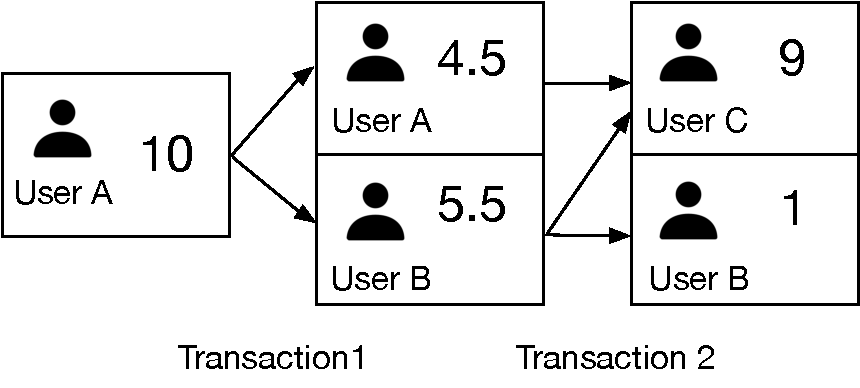
\includegraphics[width=\columnwidth]{images/UTXO.pdf}}
\caption{The Output of UTXO}
\label{fig:utxo}
\end{figure}

\textbf{Chaumian CoinJoin Mixer}
The centralized mixers have some deficiencies. Firstly, the people behind the mixer have to be trusted, so they can actually send bitcoins back. As mentioned in \ref{bitcoin-tumbler}, some scammer might build a fake mixer, when they receive money they don't send bitcoins back. Secondly, the privacy problem is not entirely solves as the mixer controller will know all the information about users.

Decentralized mixer, or the more popular name CoinJoin is a better solution, it can allow users to combine inputs and outputs from several transactions into a single big transaction. CoinJoin can solve the scam problem above, as every input require a corresponding signature from the owner, and only when all participants have signed, the transaction is accomplished and broadcast.

\textbf{Graph analysis}
As have mentioned above, bitcoin implemented UTXO to keep record,  so it is a more comprehensive way to use graph to analyse the money flow of bitcoin among addresses. Haslhofer et al.\cite{haslhofer2016bitcoin}represented GraphSense, which is a graph-centric analytics solution for digital currencies. GraphSense can be used to explore transactions and trace the flow of digital currency units, it implemented address clustering and semantic enrichment to search for paths and graph patterns within various perspectives, and it can also be used to apply anomaly detection techniques.

There are also some other previous paper which implement graph to analyse bitcoin transactions. Fleder et al.\cite{fleder2015bitcoin} annotate the public transaction graph according to some information in forums and bitcoin transaction ledger, and then revealed that the bitcoin transaction network is not entirely anonymous.
Ron et al.\cite{ron2013quantitative} and Reid et al.\cite{reid2013analysis} also use graph to analyse some features in bitcoin transactions.

However, GraphSense is a more integrated tool. It also implemented BlockSci, which is a high level of interest in blockchain analysis.


\subsection{Illicit Bitcoin Detection}
We are wishing to 